%% DONE
\let\cleardoublepage\clearpage
\chapter{Химическая технология}
\ID{IRSTI 31.23.99}{}

\begin{articleheader}
\sectionwithauthors{M.K. Kazankapova, B.T. Yermagambet, A.B. Malgazhdarova, Zh.M. Kassenova, Zh.E. Jakupova}{STUDY OF THE PHYSICOCHEMICAL PROPERTIES OF FULVIC ACID SOLUTIONS}

{\bfseries
\textsuperscript{1,2}M.K. Kazankapova\authorid,
\textsuperscript{1}B.T. Yermagambet\authorid,
\textsuperscript{1,2}A.B. Malgazhdarova\textsuperscript{\envelope }\authorid,
\textsuperscript{1}Zh.M. Kassenova\authorid,
\textsuperscript{2}Zh.E. Jakupova\authorid}
\end{articleheader}

\begin{affiliation}
\emph{\textsuperscript{1}«Institute of Coal Chemistry and Technology» LLP, Astana, Kazakhstan,}

\emph{\textsuperscript{2}L.N. Gumilyov Eurasian National University, Astana, Kazakhstan,}

\raggedright {\bfseries \textsuperscript{\envelope }}{\em Correspondent-author: malgazhdarova.ab@mail.ru}
\end{affiliation}

The article examines the extraction and purification process of fulvic
acids derived from oxidized brown coal from the Maikuben deposit using
the Forsyth method. The purification process includes stages such as
adsorption, ion exchange purification, and dialysis, with activated
carbon (Coconut) serving as the adsorbent. The physicochemical
properties of fulvic acid and its neutral dilute solutions were analyzed
using infrared (IR) and nuclear magnetic resonance (NMR) spectroscopy.
The study focused on the unique composition of fulvic acid, determining
the content of trace elements and essential organic compounds
functioning as nutrients. The reliability of the results is confirmed by
the consistency of repeated experiments and the application of
alternative analytical methods. In addition, antioxidant properties of
fulvic acid were determined, which opens up new prospects as
biologically active additives and pharmaceuticals.
Forsyth' s method has demonstrated its effectiveness,
allowing to obtain a purer product with fewer losses compared to
traditional purification methods. This approach demonstrates the
potential for developing environmentally friendly technologies for
extracting valuable substances from domestic coal resources. Further
research in this area will substantiate the specific properties and
patterns in the interaction of fulvic acid with other inorganic
compounds, and expand the potential for application.

{\bfseries Keywords:} coal, fulvic acid, membrane purification, dialysis,
adsorption, organic acids

\begin{articleheader}
{\bfseries ФУЛЬВОҚЫШҚЫЛЫ ЕРІТІНДІЛЕРІНІҢ ФИЗИКА-ХИМИЯЛЫҚ ҚАСИЕТТЕРІН ЗЕРТТЕУ}

{\bfseries
\textsuperscript{1}М.Қ. Қазанқапова,
\textsuperscript{1}Б.Т. Ермағамбет,
\textsuperscript{1,2}А.Б. Малғаждарова\textsuperscript{\envelope },
\textsuperscript{1}Ж.М. Касенова,
\textsuperscript{2}Ж.Е. Джакупова\textsuperscript{2}}
\end{articleheader}

\begin{affiliation}
\emph{\textsuperscript{1}«Көмір химиясы және технология институты» ЖШС, Астана, Қазақстан,}

\emph{\textsuperscript{2}Л.Н. Гумилев атындағы Еуразия ұлттық университеті, Астана, Қазақстан,}

\emph{е-mail: malgazhdarova.ab@mail.ru}
\end{affiliation}

Мақалада Майкөбен кен орнының тотыққан қоңыр көмірлерінен алынған
фульвоқышқылын Форсит әдісімен алу және тазарту қарастырылады. Тазарту
кезеңдері: адсорбция, иондық тазарту және диализ, мұнда адсорбент
ретінде «Кокосты» белсендірілген көмір қолданылды. Фульвоқышқылының және
оның бейтарап сұйылтылған ерітінділерінің физика-химиялық қасиеттері ИҚ
және ЯМР спектроскопиясының көмегімен талданды. Фульвоқышқылының бірегей
құрамы зерттелді, қоректік зат ретінде әрекет ететін микроэлементтер мен
маңызды органикалық қосылыстардың құрамы анықталды. Нәтижелердің
сенімділігі қайталанатын тәжірибелер мен талдаудың балама әдістерінің
ұқсастықтары кезінде қанағаттанарлық. Сонымен қатар, фульвоқышқылының
антиоксиданттық сипаттамалары анықталды, бұл биологиялық белсенді
қоспалар мен фармацевтикалық препараттар ретінде жаңа перспективаларды
ашады. Форсит әдісі дәстүрлі тазарту әдістерімен салыстырғанда аз
шығынмен таза өнім алуда өзінің тиімділігін көрсетті. Бұл тәсіл отандық
көмір ресурстарынан бағалы заттарды алудың экологиялық таза
технологияларын әзірлеудің әлеуетін көрсетеді. Бұл бағыттағы
зерттеулерді одан әрі жүргізу фульвоқышқылының басқа бейорганикалық
қосылыстармен әрекеттесуінің ерекше қасиеттері мен заңдылықтарын
негіздеуге және пайдалану мүмкіндіктерін кеңейтуге мүмкіндік береді.

{\bfseries Түйін сөздер:} көмір, фульвоқышқылы, мембраналы тазарту, диализ,
адсорбция, органикалық қышқылдар

\begin{articleheader}
{\bfseries ИЗУЧЕНИЕ ФИЗИКО-ХИМИЧЕСКИХ СВОЙСТВ РАСТВОРОВ ФУЛЬВОВОЙ КИСЛОТЫ}

{\bfseries
\textsuperscript{1}М.К. Казанкапова,
\textsuperscript{1}Б.Т. Ермағамбет,
\textsuperscript{1,2}А.Б. Малгаждарова\textsuperscript{\envelope },
\textsuperscript{1}Ж.М.Касенова,
\textsuperscript{2}Ж.Е. Джакупова}
\end{articleheader}

\begin{affiliation}
\emph{\textsuperscript{1}ТОО «Институт химии угля и технологии», Астана, Казахстан,}

\emph{\textsuperscript{2}Евразийский национальный университет им. Л.Н. Гумилева, Астана, Казахстан,}

\emph{е-mail: malgazhdarova.ab@mail.ru}
\end{affiliation}

В статье рассмотрены извлечение и очистка методом Форсита фульвовой
кислоты, полученной из окисленных из бурых углей месторождения Майкубен.
Проведены стадии очистки: адсорбция, ионная очистка и диализ, где в
качестве адсорбента использовали активированный уголь «Кокосовый».
Проанализированы физико-химические свойства методами ИК- и
ЯМР-спектроскопии фульвовой кислоты и её нейтральных разбавленных
растворов. Исследован уникальный состав фульвовой кислоты, определены
содержание основных микроэлементов, важных органических соединений,
выступающих в качестве питательных веществ. Достоверность результатов
удовлетворительная при сходимости повторных опытов и альтернативных
методов анализа. Наряду с этим, были определены антиоксидантные
характеристики фульвокислоты, что открывает новые перспективы в качестве
биологически активных добавок и фармацевтических препаратов. Метод
Форсита продемонстрировал свою эффективность, позволяя получить более
чистый продукт с меньшими потерями по сравнению с традиционными методами
очистки. Данный подход демонстрирует потенциал для разработки
экологически чистых технологий извлечения ценных веществ из
отечественных угольных ресурсов. Дальнейшие исследования в этой области
позволят обосновать специфические свойства и закономерности при
взаимодействии фульвокислоты с другими неорганическими соединениями,
расширить потенциал применения.

{\bfseries Ключевые слова:} уголь, фульвокислота, мембранная очистка,
диализ, адсорбция, органические кислоты

\begin{multicols}{2}
{\bfseries Introduction.} Currently, humic substances are in demand and are
widely produced naturally, as well as synthetically by radical
polymerization, abiotic oxidation and enzymatic methods {[}1-3{]}.

The ability of fulvic acids to enhance solubility creates potential for
the development of novel drug delivery systems and the improvement of
various pharmacological effects, such as antioxidant activity {[}4,5{]},
anti-inflammatory properties, and benefits for gastric health {[}5,6{]}.
The influence of fulvic acid on metal ion mobility in various media has
been established due to the abundance of oxygen-containing functional
groups. Water-soluble salts of fulvic acid with alkali and alkaline
earth metal cations promote their release, as well as precipitation,
dissolution, or complex formation with trivalent ions {[}7-9{]}.

Fulvic acid is an essential fraction of the organic composition of soil,
demonstrating higher chemical and physicochemical activity compared to
humic acid. The molecule of fulvic acid is small enough to overcome any
barriers in its path and contains approximately 14 quadrillion
electrons, which act as free radical scavengers. When introduced into a
biological environment, fulvic acid molecules convert accumulated waste
into nutrients and neutralize free radical waste products {[}9,10{]}.

Additionally, fulvic acid serves as a transport system capable of
delivering nutrients while binding toxins, pesticides, heavy metals,
chemical pollutants, mercury, and radionuclides into complexes {[}8{]}.

Furthermore, fulvic acids play a significant role in the acid-base
buffering capacity of soil, contributing to the retention, release, and
biological mobility of metal ions and organic chemicals within soil
matrices {[}10{]}.

Depending on their methods of extraction, fulvic acids find applications
ranging from dietary supplements to pharmaceuticals. Incorporating
fulvic acids into dietary supplements supports immune system enhancement
and protection against diseases associated with oxidative cell damage,
such as cardiovascular and oncological disorders. Due to their
antioxidant properties, fulvic acids can provide protective effects on
the cardiovascular system by neutralizing free radicals that may damage
vascular and cardiac cells. Including fulvic acids in dietary
supplements may lower the risk of atherosclerosis and inflammatory
vascular processes, making them promising for the prevention of
cardiovascular diseases such as hypertension and ischemic heart disease
{[}11-13{]}.

{\bfseries Materials and methods.} The Forsyth method was employed to
purify fulvic acid extracted from domestic brown coal from the Maikuben
deposit. Through a three-stage purification process, a high purity level
of 99\% was achieved. Commercially available coconut-based sorbents were
used as adsorbents, specifically the activated coconut charcoal
Extrasorb GAC (12x40) from India. With its high specific surface area
and sorption capacity, this charcoal effectively captured and removed
impurities, contributing to the successful purification of fulvic acids.
The characteristics of the adsorbent are presented in Table 1.
\end{multicols}

\begin{table}[H]
\caption*{Table 1 - Characteristics of coconut-based activated charcoal Extrasorb GAC (12x40)}
\centering
\begin{tblr}{
  hlines,
  vlines,
}
\textbf{Parameter}    & \textbf{Value}             \\
Particle Size         & 12x40 mesh                 \\
Specific Surface Area & \textasciitilde{}1100 m²/g \\
Iodine Number         & 1000 mg/g                  \\
Bulk Density          & 0.48 g/cm³                 \\
Hardness              & 98\%                       \\
Moisture Content      & ≤ 5\%                      \\
Ash Content           & ≤ 3\%                      \\
pH                    & 6-8                        \\
Pore Volume           & 0.55 cm³/g                 
\end{tblr}
\end{table}

\begin{multicols}{2}
The final purification stage was conducted using a membrane method
(dialysis) until a pH of 4-5 was achieved in distilled water, ensuring
complete removal of accompanying ions. By diluting the fulvic acid with
distilled water to a neutral medium, a 1.5\% model solution was
prepared.

{\bfseries Results and discussion.} The IR spectra of fulvic acids were
obtained in the Laboratory of Organometallic Chemistry and Catalysis at
Nazarbayev University (Kazakhstan) using a Nicolet iS10 FT-IR
spectrometer.

In the IR spectrum of the initial sample, distinct peaks for C=O groups
in saturated fatty acids, carboxyl, aldehyde, and ketone groups are
absent. A weak band is observed at 1635 cm⁻¹, which may indicate the
presence of C=C bonds. This suggests a low concentration of carbonyl
compounds or their strong association with other functional groups. The
broad band at 3000--3500 cm⁻¹ corresponds to OH group stretching
vibrations associated with hydrogen bonding, but it is poorly defined.
This could be due to the presence of strong intramolecular hydrogen
bonds that obscure the characteristic bands of OH groups. In the IR
spectrum of purified fulvic acid obtained using sorbent, the following
bands are clearly observed: 3600--3000 cm⁻¹, representing various OH
stretching vibrations, with sharp peaks identified approximately at
3035, 2945, and 2880 cm⁻¹. These peaks are characteristic of CH
stretching vibrations. The peak at 3035 cm⁻¹ suggests the potential
presence of aromatic CH, whereas the peaks at 2945 and 2880 cm⁻¹
indicate aliphatic CH bonds found in alkanes or alkyl groups. A
relatively small and sharp peak was detected at 2185 cm⁻¹, which falls
within the region associated with nitriles (C≡N) or cumulenes. A
moderately intense peak around 1693 cm⁻¹ indicates the presence of a
carbonyl group (C=O), which could signify ketones, aldehydes, carboxylic
acids, esters, or amides. A sharp peak at approximately 1401 cm⁻¹
suggests the presence of CH bending, likely due to CH\textsubscript{2}
bending. The obtained spectral data confirm the presence and changes in
the functional groups of fulvic acid after purification. The observation
of distinct C=O and OH group bands indicates the removal of impurities
and the improvement of the composition of the purified sample (Figure
1).
\end{multicols}

\begin{figure}[H]
    \centering
    \begin{subfigure}{0.49\textwidth}
        \centering
        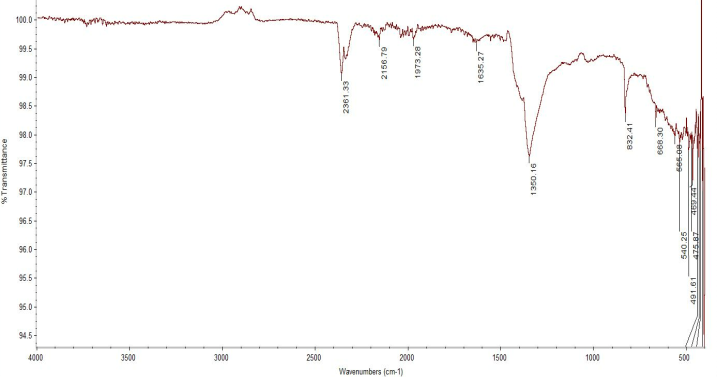
\includegraphics[width=\linewidth]{media/chem/image2}
        \caption*{Original fulvic acid derived from potassium humate}
    \end{subfigure}
    \hfill
    \begin{subfigure}{0.49\textwidth}
        \centering
        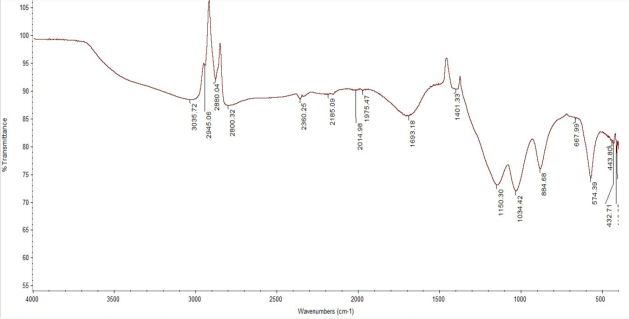
\includegraphics[width=\linewidth]{media/chem/image3}
        \caption*{Purified fulvic acid}
    \end{subfigure}
    \caption*{Fig. 1 - IR Spectra Analysis}
\end{figure}

\begin{figure}[H]
    \centering
    \begin{subfigure}{0.49\textwidth}
        \centering
        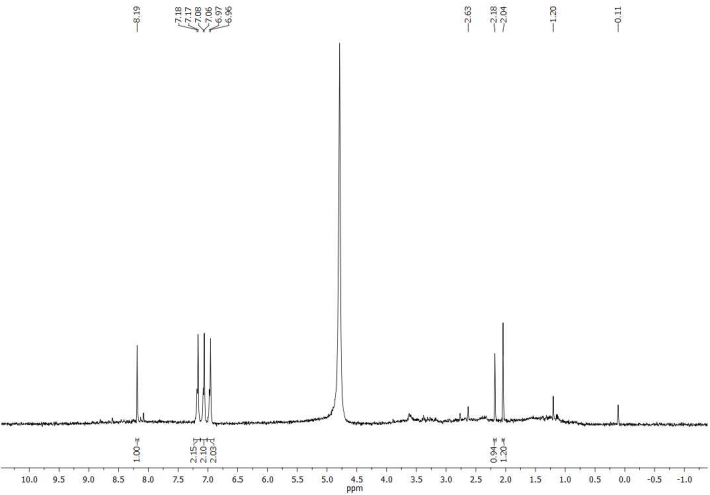
\includegraphics[width=\linewidth]{media/chem/image4}
        \caption*{Original fulvic acid derived from potassium humate}
    \end{subfigure}
    \hfill
    \begin{subfigure}{0.49\textwidth}
        \centering
        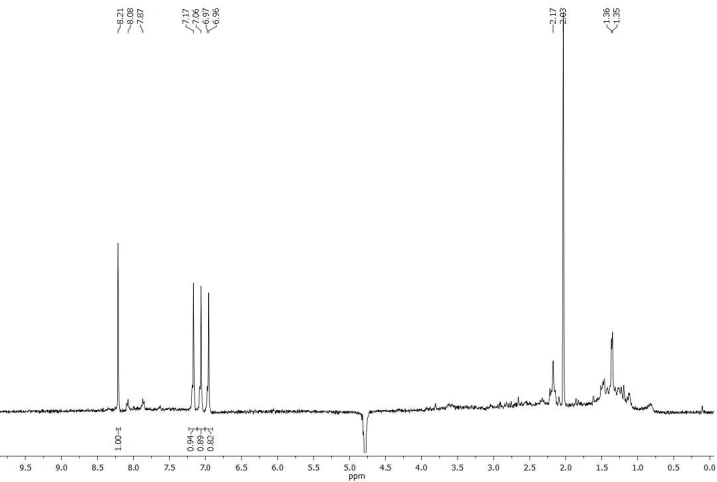
\includegraphics[width=\linewidth]{media/chem/image5}
        \caption*{Purified fulvic acid}
    \end{subfigure}
    \caption*{Fig. 2 - NMR Spectra Analysis}
\end{figure}

\begin{multicols}{2}
The NMR analysis of fulvic acid was performed using a JEOL ECA-500 MHz
NMR spectrometer. Both the unpurified and purified samples exhibit
characteristic aromatic signals in the range of approximately 6.9 to 8.2
ppm, indicating the presence of aromatic rings in the fulvic acid
structure. The shifts of aromatic protons (7.0-8.2 ppm) correspond to
substituted benzene or polycyclic aromatic systems. The complex
multiplets observed in both spectra suggest that the substitution in the
aromatic ring systems varies, with nonequivalent aromatic protons
displaying spin-spin coupling. Relative integrations imply the presence
of similar aromatic components in the two samples. The change in
relative integration suggests a modification in the chemical environment
of the aromatic protons. These shift changes likely occur as molecules
alter their interactions with one another.

The most significant difference between the spectra is observed in the
aliphatic region. The first spectrum (unpurified sample) exhibits a
broader range of signals between δ -0.1 and 3.0 ppm, indicating a higher
complexity of aliphatic components in the unpurified fulvic acid. These
signals likely correspond to varying chain lengths, branching, and
substitution patterns in the aliphatic components of the raw sample,
which probably contains other biomolecules. After purification, a
noticeable reduction in the number of signals in the aliphatic region is
observed.
\end{multicols}

\begin{table}[H]
\caption*{Table 2 - Chemical indicators of purified fulvic acid solution with "Coconut" sorbent}
\centering
\begin{tblr}{
  hlines,
  vlines,
}
Name of indicators, units of measurement                                                                               & Permissible concentrations & Results                                                    \\
1                                                                                                                      & 2                          & 3                                                          \\
{- antioxidant content, mg/dm3\\- toxic elements, mg/dm3:\\- Lead (Pb)\\- Arsenic (As)\\- Cadmium (Cd)\\- Mercury (Hg)} & {\\\\0.3\\0.1\\0.03\\0.005}    & {1356.0±0.058\\\\Not found\\Not found\\Not found\\Not found} 
\end{tblr}
\end{table}

\begin{table}[H]
\caption*{Table 3 - Chemical Indicators of the Model Solution}
\centering
\begin{tblr}{
  hlines,
  vlines,
}
{Name of indicators, \\units of measurement}                                                                                                                    & {Norm according to the \\regulatory document} & Results                                                 \\
1                                                                                                                                                               & 2                                             & 3                                                       \\
{toxic elements, mg/dm3:\\- Lead (Pb)\\- Arsenic (As)\\- Cadmium (Cd)\\- Mercury (Hg)}                                                                           & {\\0.3\\0.1\\0.03\\0.005}                       & {\\Not found\\Not found\\Not found\\Not found}            \\
{- antioxidant content, mg/dm3\\- dry matter content. \%\\- aflatoxin Bі. mg/l\\- titratable acidity, \%}                                                       & {\\\\1.0-3.5\\0.7-3.8}                            & {138.16±0.042\\Not found\\Not found\\0.24±0.02}         \\
{Pesticides, mg/kg, not more than:\\- Hexachlorocyclohexane (alpha, beta, \\gamma isomers)\\- 4,4 - dichlorodiphenyltrichloromethylmethane\\~and its metabates} & {\\0.01\\\\0.005}                                 & {\\Not found\\\\Not~found}                                  \\
{Amino acid composition, \%\\- water soluble, mg/100 g\\- B1 (thiamine chloride)\\- В3 (pantothenic acid)\\- В6 (pyridoxine)\\- Вс (folic acid)}                 &                                               & {Not found\\\\Not~found\\Not found\\Not found\\Not found} 
\end{tblr}
\end{table}

\begin{figure}[H]
	\centering
	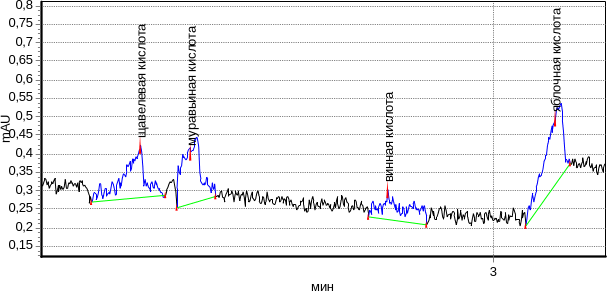
\includegraphics[width=0.8\textwidth]{media/chem/image6}
	\caption*{Fig. 3 - Chromatograms of organic acid content in the model fulvic acid solution}
\end{figure}

\begin{figure}[H]
	\centering
	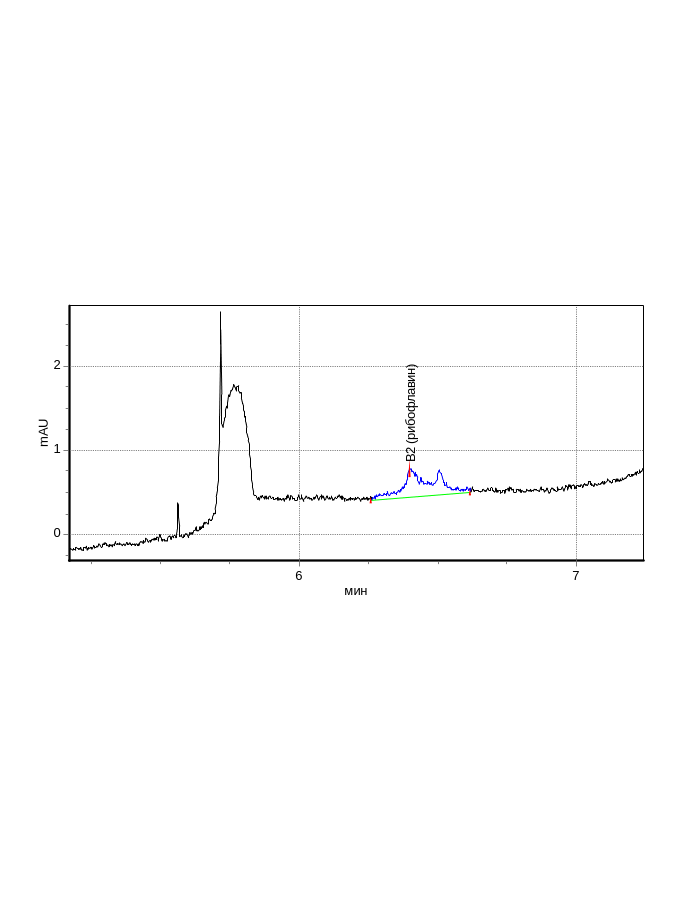
\includegraphics[width=0.8\textwidth]{media/chem/image7}
	\caption*{Fig. 4 - Chromatograms of amino acid content in the model fulvic acid solution}
\end{figure}

\begin{multicols}{2}
The second spectrum shows a pronounced singlet at δ 2.17 and a multiplet
at δ 1.36, suggesting that some aliphatic components were removed or
altered during purification. A large peak at 4.7 ppm in the unpurified
sample implies a higher content of water or residual solvent. The
inverted peak in the purified sample suggests that the sample was
saturated to suppress the signal and improve its clarity. The simplified
aliphatic region in the purified fulvic acid sample implies that the
purification process was effective in removing or altering many of the
original aliphatic components. This simplification may include the
removal of free fatty acids, carbohydrates, or other small molecular
contaminants. (Figure 2).

The results of the spectral analysis reveal significant changes in the
composition and structure of fulvic acid before and after purification.
The IR spectra indicate improved clarity of bands associated with
functional groups such as C=O and OH in the purified sample. The NMR
spectra confirm an increase in the concentration of saturated
hydrocarbon chains and a decrease in ester and alcohol groups. These
changes highlight the effectiveness of sorbents in purifying fulvic acid
and enhancing its properties.

The chemical analysis of the concentrated fulvic acid solution was
conducted using atomic absorption spectrometry to determine the levels
of toxic metals, such as lead, cadmium, mercury, and arsenic.
High-performance liquid chromatography (HPLC) methods were applied to
analyze the model solution to detect the presence of antioxidants
(Tables 2--3). The results indicated the absence of toxic elements in
the solutions and a substantial presence of antioxidants in the fulvic
acid solution, in line with the regulatory requirements of GOST
26932--86, "Raw Materials and Food Products. Methods for Determining
Toxic Element Content." The parameters of the model solution fully meet
the established standards, confirming its safety and compliance with
regulations.

The organic composition of the samples was thoroughly investigated, with
results presented in Figures 3--4. High-performance liquid
chromatography (HPLC) identified the presence of oxalic, formic,
tartaric, and malic acids in the sorption-purified fulvic acid solution.
Additionally, a small amount of vitamin B2 (riboflavin) was detected.

Thus, the obtained results of the component analysis and chemical
composition of fulvic acid and its neutral solutions contribute to the
development of sources for the production of beneficial products. The
processing of carbon-containing raw materials and the extraction of
valuable substances will significantly enhance the advancement of
efficient methods for obtaining competitive components for useful
products.

{\bfseries Conclusion.} The results indicated that the neutral solution
based on fulvic acid contains a significant amount of particularly
important organic compounds with high potential for the production of
beneficial food products.

In the future, additional physicochemical analysis of the composition of
fulvic acid extracted from coal feedstock under various conditions will
be conducted, along with a detailed examination of its antioxidant
properties.
\end{multicols}

\begin{center}
{\bfseries References}
\end{center}

\begin{references}
1. Balestrieri, F., Magrì, A.D., Magrì, A.L., Marini, D., Sacchini, A.,
Application of differential scanning calorimetry to the study of
drug-excipient compatibility// Thermochim. Acta.- 1996. - Vol. 285(2).-
P. 337-345. \href{https://doi.org/10.1016/0040-6031(96)02904-8}{DOI
10.1016/0040-6031(96)02904-8}

2. Botes, M.E., Gilada, I.S., Snyman, J.R., Labuschagne, J.P.
Carbohydrate-derived fulvic acid wellness drink: its tolerability,
safety and effect on disease markers in preART HIV-1 positive subjects
// S. Afr. Fam. Pract. - 2018. - Vol. 60 (3).- P. 91-96.

DOI 10.1080/20786190.2017.1397381

3. Chen, Y., Schnitzer, M., Scanning electron microscopy of a humic acid
and of a fulvic acid and its metal and clay complexes//Soil Sci. Soc.
Am. J.- 1996.-Vol.40(5).- P.682-686

\href{https://doi.org/10.2136/sssaj1976.03615995004000050024x}{DOI
10.2136/sssaj1976.03615995004000050024x}

4. Chien, S.J., Chen, T.C., Kuo, H.C., Chen, C.N., Chang, S.F. Fulvic
acid attenuates homocysteine-induced cyclooxygenase-2 expression in
human monocytes //BMC Compl. Alternative Med.- 2015. - Vol.15 (1). DOI
10.1186/s12906-015-0583-x

5. Francioso, O., Sanchez-Cortes, S., Tugnoli, V., Ciavatta, C., Gessa,
C. Characterization of peat fulvic acid fractions by means of FT-IR,
SERS, and 1H, 13C NMR spectroscopy // Appl. Spectrosc //1998. - Vol. 52
(2).- P. 270-277 DOI 10.1366/0003702981943347

6. Gandy, J.J., Snyman, J.R., Van Rensburg, C.E. Randomized,
parallel-group, double-blind, controlled study to evaluate the efficacy
and safety of carbohydratederived fulvic acid in topical treatment of
eczema// Clin. Cosmet. Invest. Dermatol.- 2011. -Vol.4.- P.145- 148

DOI \href{https://doi.org/10.2147/ccid.s23110}{10.2147/CCID.S23110}

7. Ahn, T., Oke, M., Schofield, A., Paliyath, G. Effects of phosphorus
fertilizer supplementation on antioxidant activities of tomato fruits.//
\href{https://pubs.acs.org/journal/jafcau?ref=breadcrumb}{Journal of
Agricultural and Food Chemistry}.2015.-Vol.53(5).-P.152-155 DOI
\href{https://doi.org/10.1021/jf040248y}{10.1021/jf040248y}

8. L.P. Canellas, F.L. Olivares, N.O. Aguiar, D.L. Jones, A. Nebbioso,
P. Mazzei, A. Piccolo. Humic and fulvic acids as biostimulants in
horticulture//Scientia Horticulturae.- 2015.-Vol. 196. -P. 15-27.
\href{https://doi.org/10.1016/j.scienta.2015.09.013}{DOI
10.1016/j.scienta.2015.09.013}

9. Y. Wang,~X. Gong,~X. Dong.~Photo-oxidation of arsenite in acidic
waters containing Suwannee River fulvic acid: roles of 3SRFA* and
hydroxyl radical //Environmental Science and Pollution Research.
-2021.-Vol.~28~(33).- P.
45144-45154.~\href{https://doi.org/10.1007/s11356-021-13900-y}{DOI
10.1007/s11356-021-13900-y}

10. Berkovic, A.M., Garcia, Einschlaq F.S., Gonzalez, M.C. at al.,
Evaluation of the Hg\textsuperscript{2+} binding potential of fulvic
acids from fluorescence excitation-emission matrices //Photochem.
Photobiol. Sci.- 2013. -Vol.12. - P. 384 - 392. DOI
\href{https://doi.org/10.1039/c2pp25280e}{10.1039/c2pp25280e}

11. W. Tang, G. Zeng, J. Gong, J. Liang, P. Xu, C. Zhang, B. Huang.
Impact of humic/fulvic acid on the removal of heavy metals from aqueous
solutions using nanomaterials: A review. //Science of the Total
Environment.- 2014.-Vol. 468-469.- P.1014-1027.

\href{https://doi.org/10.1016/j.scitotenv.2013.09.044}{DOI
10.1016/j.scitotenv.2013.09.044}

13. W. Ding,~T.E. Romanova,~I.P. Pozdnyakov,~V.A. Salomatova,~M.V.
Parkhats,~B.M. Dzhagarov,~E.M. Glebov,~F. Wu,~O.V.
Shuvaeva.~Photooxidation of arsenic (III) in the presence of fulvic
acid//~Mendeleev Communications.-2016. - Vol.~26~(3).- P. 266-268.~

\href{https://doi.org/10.1016/j.mencom.2016.05.016}{DOI
10.1016/j.mencom.2016.05.016}
\end{references}

\begin{authorinfo}
\emph{{\bfseries Information about the authors}}

Kazankapova M.K. - PhD , assoc. professor, member correspondent of the
KazNANS, Leading Researcher, Head of Laboratory of LLP «Institute of
Coal Chemistry and Technology», Astana, Kazakhstan, e-mail:
maira\_1986@mail.ru;

Yermagambet B.T. - Doctor of Chemical Science, rofessor, Academician of
the KazNANS, Project Manager, Chief Researcher, Director of LLP
«Institute of Coal Chemistry and Technology», Astana, Kazakhstan,
e-mail: bake.yer@mail.ru;

Malgazhdarova A.B.- master student Eurasian National University of L.N.
Gumilyov, Junior Researcher «Institute of Coal Chemistry and
Technology», Astana, Kazakhstan, e-mail:
\href{mailto:malgazhdarova.ab@mail.ru}{\nolinkurl{malgazhdarova.ab@mail.ru}};

Kassenova Z.M.- Сandidate of Technical Sciences (PhD), Leading
Researcher LLP «Institute of Coal Chemistry and \\Technology», Astana,
Kazakhstan, e-mail:
\href{mailto:zhanar_k_68@mail.ru}{\nolinkurl{zhanar\_k\_68@mail.ru}};

Jakupova Zh.E. - Candidate of Chemical Sciences, associate Professor
Eurasian National University of L.N. Gumilyov, Astana, Kazakhstan,
e-mail: zhanereke@mail.ru

\emph{{\bfseries Сведения об авторах}}

Казанкапова М. К. -PhD, асс. профессор, чл.-корр. КазНАЕН, ведущий
научный сотрудник, заведующий лабораторией ТОО «Институт химии угля и
технологии», Астана, Казахстан, e-mail: maira\_1986@mail.ru;

Ермагамбет Б.Т.-доктор химических наук, профессор, академик КазНАЕН,
руководитель проекта, главный научный сотрудник, директор ТОО «Институт
химии угля и технологии», Астана, Казахстан, e-mail: bake.yer@mail.ru;

Малгаждарова А. Б.- магистрант Евразийского национального университета
им. Л.Н. Гумилева, младший научный сотрудник ТОО «Институт химии угля и
технологии», Астана, Казахстан, e-mail:
\href{mailto:malgazhdarova.ab@mail.ru}{\nolinkurl{malgazhdarova.ab@mail.ru}};

Касенова Ж. М.- кандидат технических наук (PhD), ведущий научный
сотрудник ТОО «Институт химии угля и технологии», Астана, Казахстан,
e-mail:
\href{mailto:zhanar_k_68@mail.ru}{\nolinkurl{zhanar\_k\_68@mail.ru}};

Джакупова Ж.Е. - кандидат химических наук, доцент кафедры химии
Евразийский национальный университета им. Л.Н. Гумилева, Астана,
Казахстан, e-mail: zhanereke@mail.ru
\end{authorinfo}
